\label{chapter:ModelBuild}
This model build workflow
is designed to create and fine-tune a \mfus\ model, which represents a conceptual model we have of some hydrogeologic flow system, real or imaginary. \mut, provides the link between conceptual model and \mfus\ model, and is intended to minimize the amount of time we spend building and testing it.
    \footnote{As you read along, we urge you to you carry-out the workflow steps we describe here. Hands-on experience is probably the best way to learn how to use new software. You can modify our workflow to suit yourself, with the goal always being to save more of your valuable time and energy!}


The first step in the workflow is to define the conceptual model.  To illustrate a typical model build,  we'll adopt a simple conceptual example.
    \footnote{This example is described in Section~\ref{section:1d_column_example}.}
of groundwater flow though a 1D column of soil that is 100 m thick and which receives a constant rainfall of 0.4 m/yr, and where the groundwater table is fixed at the base of the column.

Next we need to develop a \mut\ input file, which is a plain ascii text file that you can edit with your preferred editor (e.g. Windows Notepad). \footnote{Our personal favourite editor is WinEdt (\url{https://www.winedt.com/snap.html}).}
Each modflow input file name must have the extension \texttt{mut}, and a prefix of your choice. Examples of valid \mut\ input file names are \texttt{\_build.mut} or \texttt{good.mut}. Most often, the easiest approach is to copy an existing input file and modify it as required.  This helps reduce set-up time and avoid potential errors that are introduced when creating input files from scratch.

We recommend you copy the contents of the folder \texttt{MUT\_Examples$\backslash$1\_VSF\_Column} to a new location (e.g.\ \texttt{C:$\backslash$SandBox}) and perform the actions yourself as we move through the workflow.  If you do so, your working directory will look something like this:
    \vspace{.2in} \\
    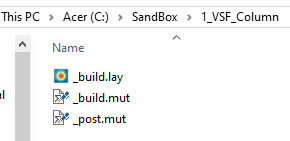
\includegraphics[width=0.4\textwidth]{vsf_column_folderinit}
    \vspace{.2in} \\
In this example, there are two \mut\ input files, one for the model build called \texttt{\_build.mut}, and one for post-processing called \texttt{\_post.mut} (discussed later in chapter~\ref{texfile:ModelExecution}).



\pagebreak
\mut\ tries to obtain a prefix in one of these three ways:
\begin{enumerate}
    \item \textbf{As a command line argument:} \label{commarg} At the command prompt, \mut\ checks for the presence of a command line argument.  For example, typing this:
\begin{verbatim}
    mut  MyInput
\end{verbatim}
        would cause \mut\ to process the input file \texttt{MyInput.mut}.
    \item \textbf{Use a prefix file:} If there is no command line argument, \mut\ checks for the presence of the file \texttt{mut.pfx} in the folder.  If present, \mut\ will read the prefix from it. For example, if the mut file was called \texttt{\_build.mut} then the file \texttt{mut.pfx} would have the single line \texttt{\_build}.
    \item \textbf{Use the default input file name:} Finally, if there is no command line argument or \texttt{mut.pfx} file in the folder, \mut\ checks for the presence of the file \texttt{a.mut}.  If present in the folder, \mut\ will use it.
\end{enumerate}
If none of these methods are successful, \mut\ will then prompt you for a prefix as shown here:
        \vspace{.2in} \\
        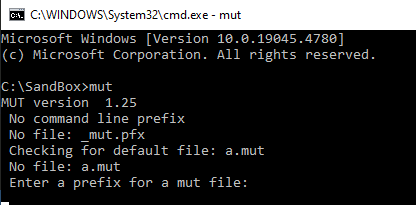
\includegraphics[width=0.6\textwidth]{mut_no_prefix}
        \vspace{.2in} \\




 In our example, we will use option~\ref{commarg}.  First, start a command prompt in the folder \texttt{C:$\backslash$1\_VSF\_Column$\backslash$SandBox} as follows:
\begin{enumerate}
    \item  Navigate to the folder in File Explorer.
   \item  Click on the path in File Explorer:

        
\includegraphics[width=0.2\textwidth]{HighlightPath}

    \item  Replace the existing path with the string 'cmd':

        
\includegraphics[width=0.4\textwidth]{cmd}

    \item Press Enter/Return and you will see the following command prompt:

        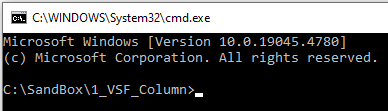
\includegraphics[width=0.4\textwidth]{cmdPrompt}

\end{enumerate}

Now start \mut\ by typing:
\begin{verbatim}
    mut  _build
\end{verbatim}
Note the following as \mut\ processes the input file:
\begin{itemize}
    \item Output is written both to the screen and to the file \verb+_buildo.eco+ as execution progresses.  The first thing \mut\ writes is the version number, which can be checked if something unexpected happens. If the run is successful the last line written will be \texttt{Normal exit}, otherwise an error message will be given.
    \item  Comment lines are stripped from the input file and echoed to the screen and file.
    \item  Several new output files are created:
        \vspace{.2in} \\
        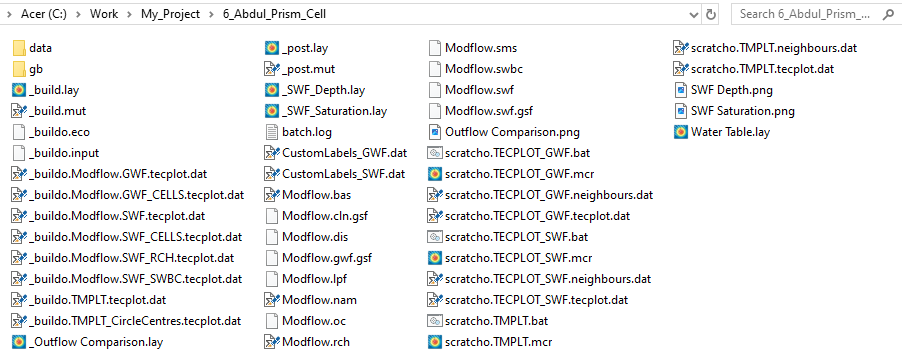
\includegraphics[width=0.8\textwidth]{buildFiles}
        \vspace{.2in} \\
    \item \mut\ output files have the prefix \texttt{\_buildo}.  Because we started the prefix with the underscore character,  output files appear near the start of the list if sorted by name.
    \item There are several \tecplot\ output files that are indicated by the suffix \texttt{.tecplot.dat}.
    \item Modflow files are written using the default prefix \texttt{Modflow}, (e.g.\ \texttt{Modflow.nam, Modflow.bas} etc.)  The prefix can be customized if desired but there are advantages to keeping this 'generic' one, such as portability of post-processing scripts or \tecplot\ layout files that follow this generic naming convention.
    \item Several scratch files (with prefix \texttt{scratcho}) are written which may be useful for debugging during, for example, code development.  These can be ignored in most cases.
    \item \mut\ deletes previously generated output files and writes a fresh set each time it is run.  This prevents confusion that can arise when out-of-date output files are present.
        \footnote{For example, if we define a recharge boundary condition, \mut\ will create the file \texttt{\textit{prefix}o.Modflow.SWF\_RCH.Tecplot.dat} which shows the locations and recharge values assigned to Modflow cells.  If we then removed the recharge condition from the input file, but did not delete this output file, it may lead us to think that recharge condition is still being applied.}
\end{itemize}


We will now go through the contents of the example input file \texttt{\_build.mut}. Open the file \texttt{MUT\_Examples$\backslash$1\_VSF\_Column$\backslash$\_build.mut} in your preferred text editor.

You will see the first couple of lines are comments describing the problem:
\begin{verbatim}
    ! Examples\1_VSF_Column:
    !   A modflow project of a 1D column generated from a simple 2d rectangular mesh
\end{verbatim}
Comments begin with an exclamation point character '!' and are ignored by \mut.  \mut\ initially strips the input file of all comments and creates a clean copy called \textit{prefix}\verb+o.input+, which is then processed by \mut.

In addition to comments, the input file contains \mut\ instructions.  Some instructions require additional data, which can be numbers or alphanumeric strings.
The next line in the input file is the instruction:
\begin{verbatim}
    build modflow usg
\end{verbatim}
This instruction starts what we refer to as a subtask.  Each subtask has it's own set of instructions, which are read until an \texttt{end} card is encountered, which teminates the processing of the subtask.  We suggest appending the subtask name to the \texttt{end} instruction, which makes debugging easier when subtasks are nested.  So for example, we would end this subtask with the following instruction:
\begin{verbatim}
    end build modflow usg
\end{verbatim}


The steps required to build a \mfus\ GWF model with \mut\ are:
\begin{itemize}
    \item Define a template mesh.
    \item Generate a 3D GWF domain from the template mesh.
    \item Assign material properties to the GWF domain.
    \item Assign the boundary and starting conditions.
    \item Assign the stress period and time-stepping parameters.
    \item Assign the solver parameters.
    \item Assign the output controls.
\end{itemize}

The following sections describe the rest of the input file contents.

